\section{Diseño}
\label{sec:diseno}

Una vez presentado el contexto, los objetivos, así como las herramientas empleadas,
en este capítulo se detalla la mejora desarrollada sobre la herramienta scracth4robots.
Primero presentaremos el diseño global y después analizaremos en detalle que aportaciones se han realizado y como se han llevado a cabo.

Para englobar todos los componentes ya definidos en un mismo contexto vamos a definir la arquitectura y diseño de la herramienta.\\

\begin{figure}[H]
    \centering
    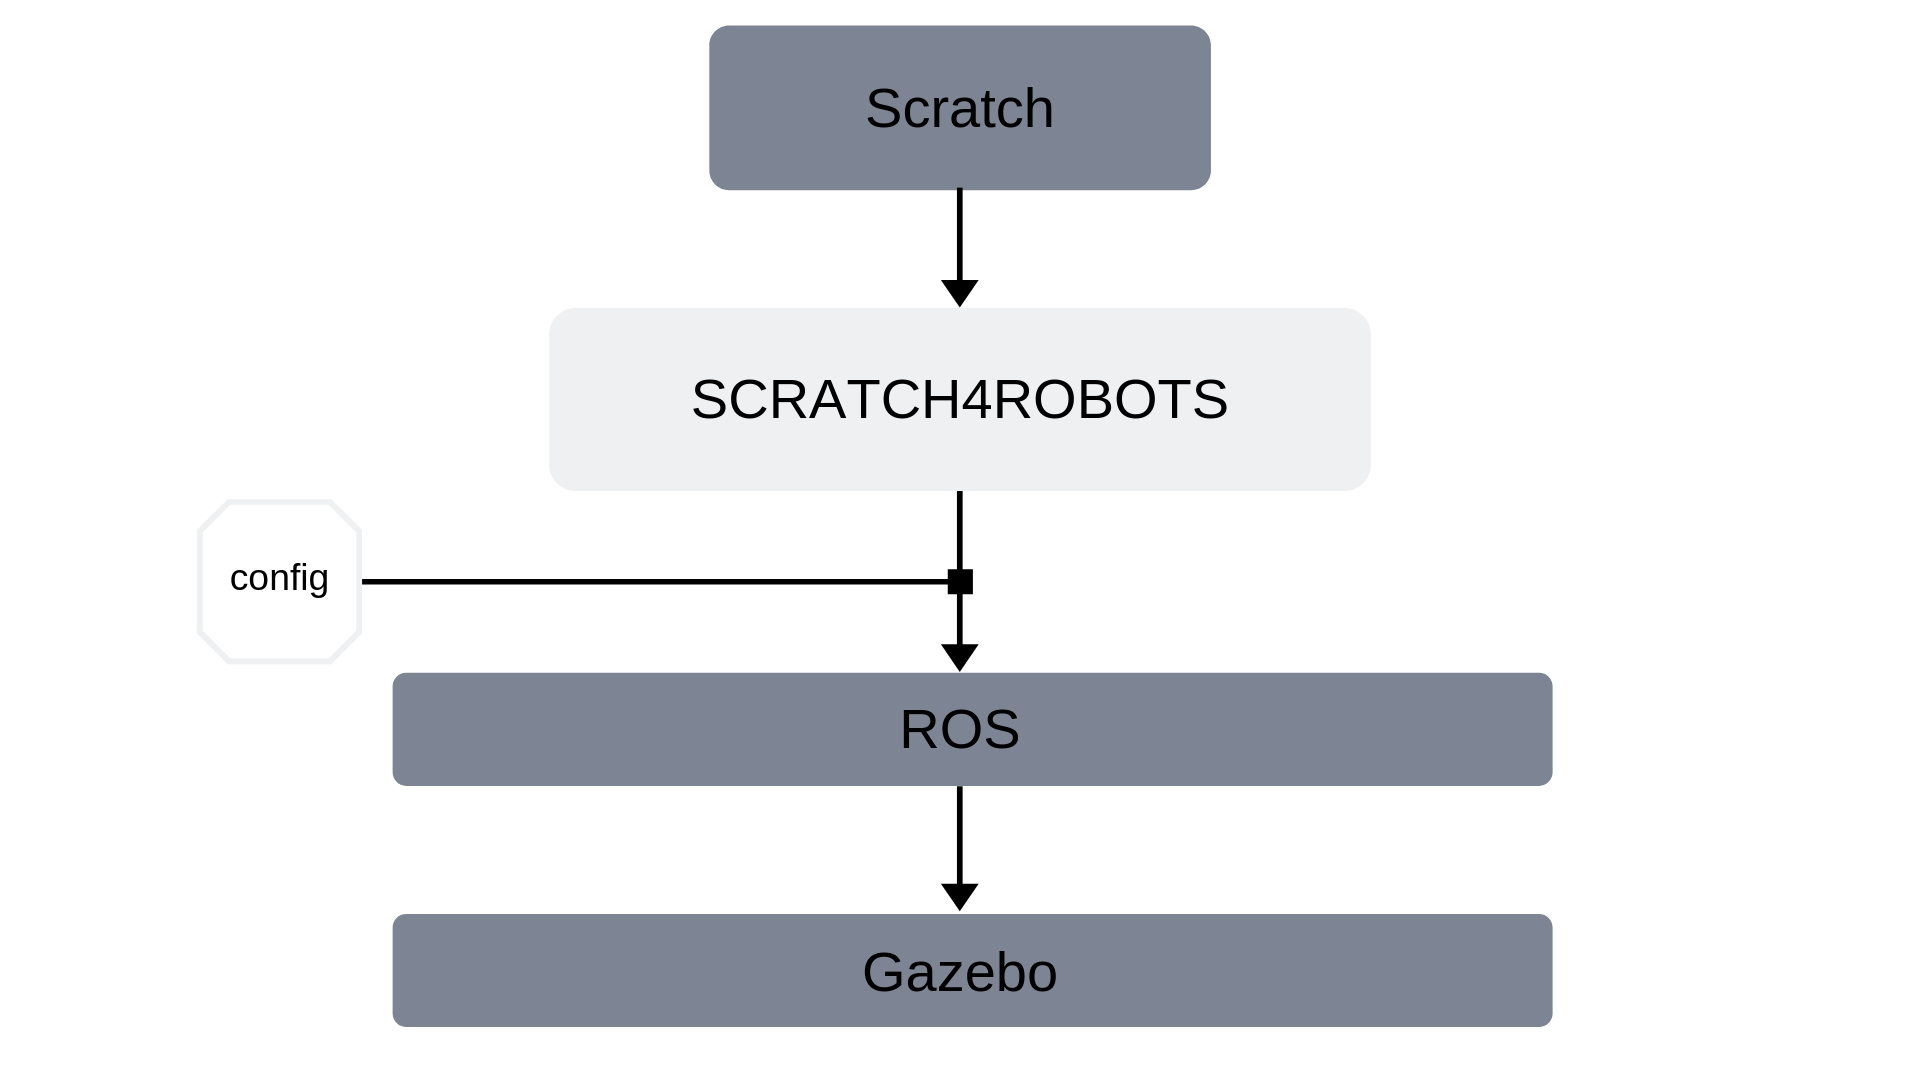
\includegraphics[scale=0.30]{img/diseno.jpg}
  	\caption{Diseño de scratch4robots}
  	\label{fig:s4r}
\end{figure}

Partimos de un proyecto generado en el lenguaje de programación visual Scratch, al que se le ha agregado una serie de bloques robóticos, definidos e implementados por nosotros. Con estos nuevos bloques y los ya disponibles en Scratch se programará la lógica que queremos que siga nuestro robot.\\

Una vez tenemos nuestro proyecto, Scratch4Robots se encarga de la traducción de este proyecto a un nodo ROS, programado en Python, que con un único fichero de configuración en el que indicamos los tópicos que vamos a necesitar, se encuentra listo para su ejecución sobre un robot en un entorno simulado, por ejemplo Gazebo.\\

Una vez lanzado el nodo habremos sido capaces de aplicar una lógica programada en Scratch sobre un robot en un entorno simulado.


\section{Desarrollo de bloques}
\label{sec:desarrollo-de-bloques}

Una de las aportaciones de este trabajo a la herramienta ha sido la refactorización de bloques ya existentes y la agregación de nuevos bloques funcionales.
En la programación visual entendemos por bloque a cada componente visual que contiene una lógica específica, con la agrupación de bloques podemos conseguir un flujo de programación complejo. En primer lugar vamos a describir como agregar estos nuevos bloques a Scratch, siguiendo con su definición e implementación.

\subsection{Extensión de Scratch}

Scratch facilita el uso de bloques personalizados mediante extensiones externas, estas  extensiones externas a la aplicación se definen mediante el uso de ficheros JSON, aunque por convención, en Scratch tendrán extensión .s2e. Este tipo de ficheros se creó para la comunicación mediante HTTP de bloques con aplicaciones auxiliares, por ejemplo algún tipo de hardware. Nosotros no vamos a utilizar esta funcionalidad, únicamente nos ayudamos de este documento .s2e para definir nuestra extensión y pueda ser usada desde el IDE offline de scratch.\\

En este documento se define un objeto JSON, el cual será la definición de la extensión, en el que se incluye el nombre de la extensión, un puerto usado para la comunicación de componentes externos en caso de ser necesario y una lista de bloques de Scratch. \\

A continuación se define un ejemplo de una extensión para Scratch. 
\begin{lstlisting}[language=json,firstnumber=1]
{ 
  "extensionName": "Extension Example",
  "extensionPort": 12345,
  "blockSpecs": [
    [" ", "beep", "playBeep"],
	[" ", "set beep volume to %n", "setVolume", 5],
	["r", "beep volume", "volume"],
  ]
}
\end{lstlisting}

El campo ``blockSpecs'' describe los bloques de extensión que aparecerán en el apartado ``Más bloques'' en la aplicación de Scratch.
En en este caso, hay tres bloques:
\begin{itemize}
\item Un bloque de comandos que reproduce un pitido.
\item Un bloque de comando que
establece el volumen del pitido.
\item Un bloque que devuelve un valor, que informa del volumen de un pitido.
\end{itemize}

Cada bloque se describe mediante una matriz con los siguientes campos:
\begin{itemize}
\item \textbf{Tipo de bloque}:

\begin{itemize}
\item ' ' - bloque de comandos
\item 'w' - bloque de comandos que esperan
\item 'r' - bloque que retorna un valor
\item 'b' - bloque que retorna un booleano 
\end{itemize}
\item \textbf{Formato de bloque}:

El formato de bloque es una cadena que describe las etiquetas y ranuras de parámetros que aparecen en el bloque.
Las ranuras de parámetros están indicadas por una palabra que comienza con '\%' y puede ser una de:
\begin{itemize}
\item \%n -  parámetro de número 
\item \%s - parámetro de cadena 
\item \%b - parámetro booleano
\end{itemize}
\item \textbf{Operación o nombre de variable remota}:

El campo de operación en una especificación de bloque se usa de dos maneras. Para bloques de comandos, se envía a la aplicación auxiliar, junto con cualquier valor de parámetro, para invocar una operación. O para retornar bloques, es el nombre de una variable de sensor. Los valores de la variable del sensor se guardan en un diccionario.
La ejecución de un bloque simplemente devuelve el valor reportado más recientemente para esa variable de sensor.
\item \textbf{Parámetros predeterminados}:

Se pueden añadir cero o más valores de parámetros predeterminados

\item \textbf{Menús desplegables}:

Los bloques que definimos pueden hacer uso de parámetros de menú, los cuales definiremos de dos formas:
\begin{itemize}
\item \%m.menuName - parámetro de menú (no editable), proporciona un sencillo espacio para los parámetros del menú desplegable.
\item \%d.menuName - parámetro de número editable con menú, proporciona una ranura de parámetro numérico con un menú auxiliar.
\end{itemize}
\end{itemize}

Con todo esto podemos entender la definición de alguno de nuestros bloques como podemos en el siguiente extracto de código, en el que se ve la definición de algunos de nuestros bloques.
\begin{nobreak} 
\begin{lstlisting}[language=json,firstnumber=1]
{
  "extensionName": "Scratch4Robots",
  "extensionPort": 12345, 
  "blockSpecs": [
    ["", "stop robot-drone", "stop"],         
    ["", "move robot %m.robotDirections speed %n", "robot/move/speed", "forward", 1],
    ["r", "color detection %m.color", "camera/all","red"],
    ["r", "frontal laser distance", "laser/frontal"],
  ],
  "menus": {
    "robotDirections": ["forward", "back"],         
    "color": ["red", "blue"]
  }
}

\end{lstlisting}
\end{nobreak} 

\subsection{Bloques genéricos}
Antes de comenzar con los bloques propios a nuestra extensión vamos a necesitar una serie de bloques genéricos que nos ayuden a realizar lógica básica de programación como pueden ser operadores matemáticos, operadores lógicos y sentencias básicas de programación. Scratch ya nos ofrece estos bloques por definición, por lo que no hará falta agregarlos a nuestra extensión específica, solamente nos encargaremos de su posterior traducción a código Python.\\

A continuación mostramos todos los bloques genéricos de los que podemos hacer uso desde la herramienta Scratch4Robots, ya que hemos implementado su traducción a Python.

\begin{figure}[H]
	\begin{minipage}{0.33\textwidth}
    	\centering
    	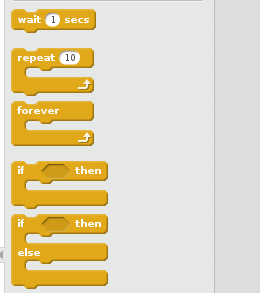
\includegraphics[scale=0.40]{img/bloques-control.png}
     	\caption{Bloques de control}
  		\label{fig:bloques-control}
   	\end{minipage}\hfill
   	\begin {minipage}{0.33\textwidth}
     	\centering
     	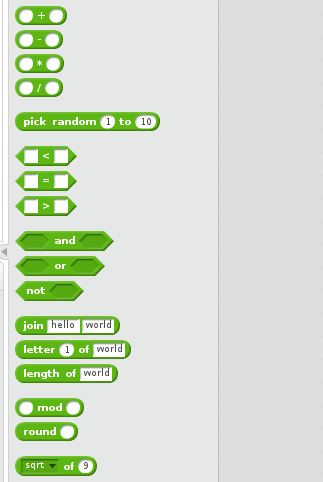
\includegraphics[scale=0.40]{img/bloques-mat.png}
  		\caption{Bloques matemáticos y lógicos}
  		\label{fig:bloques-mat}
	\end{minipage}
	\begin {minipage}{0.33\textwidth}
     	\centering
     	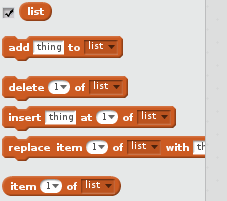
\includegraphics[scale=0.40]{img/bloques-listas.png}
     	\caption{Bloques de listas}
     	\label{fig:bloques-listas}
	\end{minipage}
\end{figure}

\begin{itemize}
\item \textbf{Bloques de operadores matemáticos}:
Bloques fundamentales de cara a realizar una lógica posterior con los datos obtenidos desde los sensores de nuestros robots, estos bloques son una de las mejoras ofrecidas por este trabajo.
	\begin{itemize}

    \item \textbf{sqrt of ()}: Realiza la operación raíz cuadrada de un número dado
    \item \textbf{sin of ()}: Realiza la operación seno de un número dado
    \item \textbf{cos of ()}: Realiza la operación coseno de un número dado
    \item \textbf{tan of ()}: Realiza la operación tangente de un número dado
    \item \textbf{asin of ()}: Realiza la operación arcoseno de un número dado
    \item \textbf{acos of ()}: Realiza la operación arcocoseno de un número dado
    \item \textbf{atan of()}: Realiza la operación arcotangente de un número dado
    \item \textbf{log of ()}: Realiza la operación logaritmo de un número dado
    \item \textbf{ln of ()}: Realiza la operación logaritmo neperiano de un número dado
    \item \textbf{abs of ()}: Devuelve el valor absoluto de un número
    \item \textbf{mod of ()}: Devuelve el módulo de un número dado
    \end{itemize}

\item \textbf{Bloques de operadores lógicos}:
Permiten construir expresiones lógicas, se obtiene como resultado booleanos.
\begin{itemize}

 \item \textbf{And}: Operador de conjunción.
 \item \textbf{Or}: Operador de disyunción.
 \item \textbf{NOT}: Operador de negación.
 \item \textbf{Mayor que y Menor que}: Operadores de comparación numérica.
\end{itemize}

\item \textbf{Bloques de control}:
Estructuras de control básicas de programación.
\begin{itemize}
\item \textbf{Wait () secs}: Pausa la ejecución el tiempo especificado, equivalente a la sentencia \textit{time.sleep()} de Python.
\item \textbf{Forever}: Bucle infinito, equivalente a \textit{while(True)} en lenguaje Python.
\item \textbf{If () then}: Comprueba la condición para que si la condición es verdadera, los bloques dentro de ella se ejecuten.
\item \textbf{If () Then, Else}: Comprueba la condición para que si la condición es verdadera, los bloques dentro de la primera condición se activen y si la condición es falsa, los bloques dentro de la segunda condición se activarán.
\item \textbf{Repeat ()}: Un ciclo que repite la cantidad de veces especificada, sería la equivalencia al bucle \textit{for} en Python.
\end{itemize}
\item \textbf{Otros}
\begin{itemize}

\item \textbf{say ()}: Imprime lo que le añadas como argumento, equivalente a \textit{print}.
\item \textbf{Set () to ()}: Utilizado para dar valor a una variable en concreto.
\end{itemize}

\item \textbf{Bloques de listas}:
Esta serie de bloques desarrollados en esta versión han sido de gran ayuda a la hora de la refactorización y creación de otros bloques de mayor complejidad.
\begin{itemize}
\item \textbf{Insert () at () of ()}: Inserta elemento en la posición seleccionada de la lista indicada.
\item \textbf{Item () of ()}: Devuelve el elemento almacenado en la posición indicada de la lista.
\item \textbf{Add () to ()}: Inserta en la lista un elemento.
\item \textbf{Delete () of ()}: Elimina el elemento en una posición determinada de la lista.
\end{itemize}
\end{itemize}

\subsection{Bloques para drones}
Estos bloques ya pertenecen a la extensión creada para la herramienta.
En este trabajo se ha realizado una refactorización completa de todos los bloques referentes a drones y la agregación de nuevos bloques. 
\begin{itemize}
\item \textbf{Bloques perceptivos}:
Nos permiten obtener información de sensores incorporados en el drone.
	\begin{itemize}
	\item \textbf{Get pose3D}: Obtiene el valor de la posición 3D del robot
	\item \textbf{Color detection}: Nuevo componente añadido en esta versión, que haciendo uso de una cámara en el robot, detecta objetos de un determinado color, introducido como argumento, devolviendo una lista que contendrá las posiciones en los ejes x,y y el tamaño del objeto, en la imagen capturada por la cámara. 
	\end{itemize}
\item \textbf{Bloques de movimiento}
	\begin{itemize}
	\item \textbf{Stop robot-drone}: Pone a su valor inicial todas las velocidades del robot.
	\item \textbf{Drone take off}: Hace que el drone despegue.
	\item \textbf{Drone land}: Realiza un aterrizaje controlado del drone.
	\item \textbf{Move drone}: Bloque que tras la refactorización admite una lista con las velocidades del drone en los diferentes ejes (velocidad en el eje x, velocidad en el eje y, velocidad yaw).
	\end{itemize}
\end{itemize}

Cabe destacar de estos bloques que una vez traducidos al nodo final, que se consigue implementar el funcionamiento de drones bajo el middleware ROS, algo elaborado en este trabajo.\\

Para ello nos apoyamos en MAVROS\footnote{\url{http://wiki.ros.org/mavros}}, puente oficial entre nodos ROS y Mavlink\footnote{\url{https://github.com/mavlink}}, el protocolo de comunicación estándar para drones.

\subsection{Bloques para robots con ruedas}
\begin{itemize}
\item \textbf{Bloques perceptivos}
	\begin{itemize}
	\item \textbf{Pose3D} :Obtiene el valor de la posición 3D del robot.
	\item \textbf{Color detection}: Bloque homólogo al del drone, dado un color nos devuelve.
	\item \textbf{Frontal distance}: Obtiene la medida promedio de los datos del láser frontal. 
	\end{itemize}
\item \textbf{Bloques de movimiento}
	\begin{itemize}

	\item \textbf{robot move ()}: Admite como parámetro una lista con las velocidades en el eje x e y.
	\item \textbf{robot move () to position ()}: Bloque de lógica similar al anterior, por el contrario este bloque no usa listas, por lo que únicamente admite una velocidad en una dirección.
	\item \textbf{robot turn ()} Permite la rotación sobre el propio eje del robot.

	\end{itemize}
\end{itemize}

\begin{figure}[H]
    \centering
    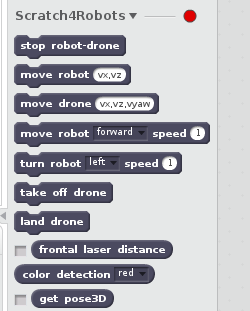
\includegraphics[scale=0.75]{img/bloques-s4r.png}
  	\caption{Bloques propios de la extensión Scratch4Robots}
  	\label{fig:curiosity}
\end{figure}


\section{Traducción de bloques}
El último paso será definir la estrategia que vamos a seguir para realizar la traducción de los bloques creados anteriormente, al nodo ROS final, programado en Python.

Vamos a estudiar más a fondo como trabaja la biblioteca Kurt y cómo nos ha ayudado en la traducción de bloques.\\

Kurt es una biblioteca de Python que permite la manipulación compleja de proyectos Scratch (archivos .sb o .sb2) a través de simples comandos de Python. Incluye un decompilador, que permite que un proyecto se cargue en un conjunto de objetos de Python, y un compilador que permite el empaquetamiento de un conjunto de scripts de imágenes / texto en proyectos scratch.\\

En este proyecto se ha utilizado una versión\footnote{\url{https://pypi.org/project/jderobot-kurt/}} mejorada de esta biblioteca, con ciertas adaptaciones para el tratamiento de extensiones externas como la nuestra. Kurt define los bloques usados por Scratch como objetos JSON, en esta nueva versión se agrega un fichero con la configuración de nuestros bloques como objetos JSON. De esta forma se agrega la capacidad de obtener la información de los bloques de nuestra extensión.\\

La clase principal de kurt almacena el contenido de un archivo de proyecto Scratch.
Los contenidos incluyen variables globales y listas, el escenario y los sprites, cada uno con sus propios scripts, sonidos, variables y listas.\\

Una vez obtenido el contenido de un proyecto Scratch en un objeto Python, con el siguiente fragmento de código somos capaces de obtener el String representativo de cada bloque.\\

\begin{lstlisting}[language=python,firstnumber=1]
# load the scratch project
p = kurt.Project.load(open_path + sys.argv[1])

# show the blocks included
for scriptable in p.sprites + [p.stage]:
	for script in scriptable.scripts:
		# exclude definition scripts
		if "define" not in script.blocks[0].stringify():
			s = script
print("Stringify:")
sentences = []
for b in s.blocks:
	print(b.stringify())
\end{lstlisting}

Una vez tenemos la lista de los Strings equivalentes a los bloques del proyecto Scratch, hay que realizar una tarea de transformación de estas a código Python.\\

En este trabajo se modifica de forma notable la forma en la que se realizaba de forma inicial esta traducción, agregando una gran cantidad de bloques soportados y añadiendo un grado de recursividad que permite la traducción de bloques anidados.\\

En la traducción nos apoyamos de unos diccionarios Python en los que mapeamos el string equivalente al bloque Scratch con el equivalente Python que queremos sustituir, esto nos lleva al último punto de nuestro desarrollo. Para ciertos bloques de Scratch existe una traducción directa a un comando Python como ya hemos visto antes. Mientras que para los bloques robóticos definidos por nuestra extensión debemos de crear un método específico que contenga toda la lógica a implementar.\\

En este trabajo hemos refactorizado la totalidad de la lógica tras los bloques robóticos, dándole una mayor coherencia a todos ellos. Además de crear lógica completamente nueva para ciertos bloques agregados en esta versión. Cabe destacar el bloque referente a la detección de objetos de un cierto color.\\

Usando la biblioteca OpenCV de Python y con técnicas de análisis computacional de imágenes, de una simple imagen somos capaces de obtener su posición en la imagen y su tamaño.\\

Además de la traducción, Scratch4Robots encapsula este código Python en un nodo ROS, que contiene todo lo necesario para su posterior ejecución, con el único requisito de un fichero de configuración en el que especificaremos los tópicos que va a necesitar nuestro nodo. Cerrando de esta forma el ciclo de trabajo de la herramienta.\\